\chapter{Ergebnisaufnahmen}
\begin{sidewaysfigure}[h]
  \centering
	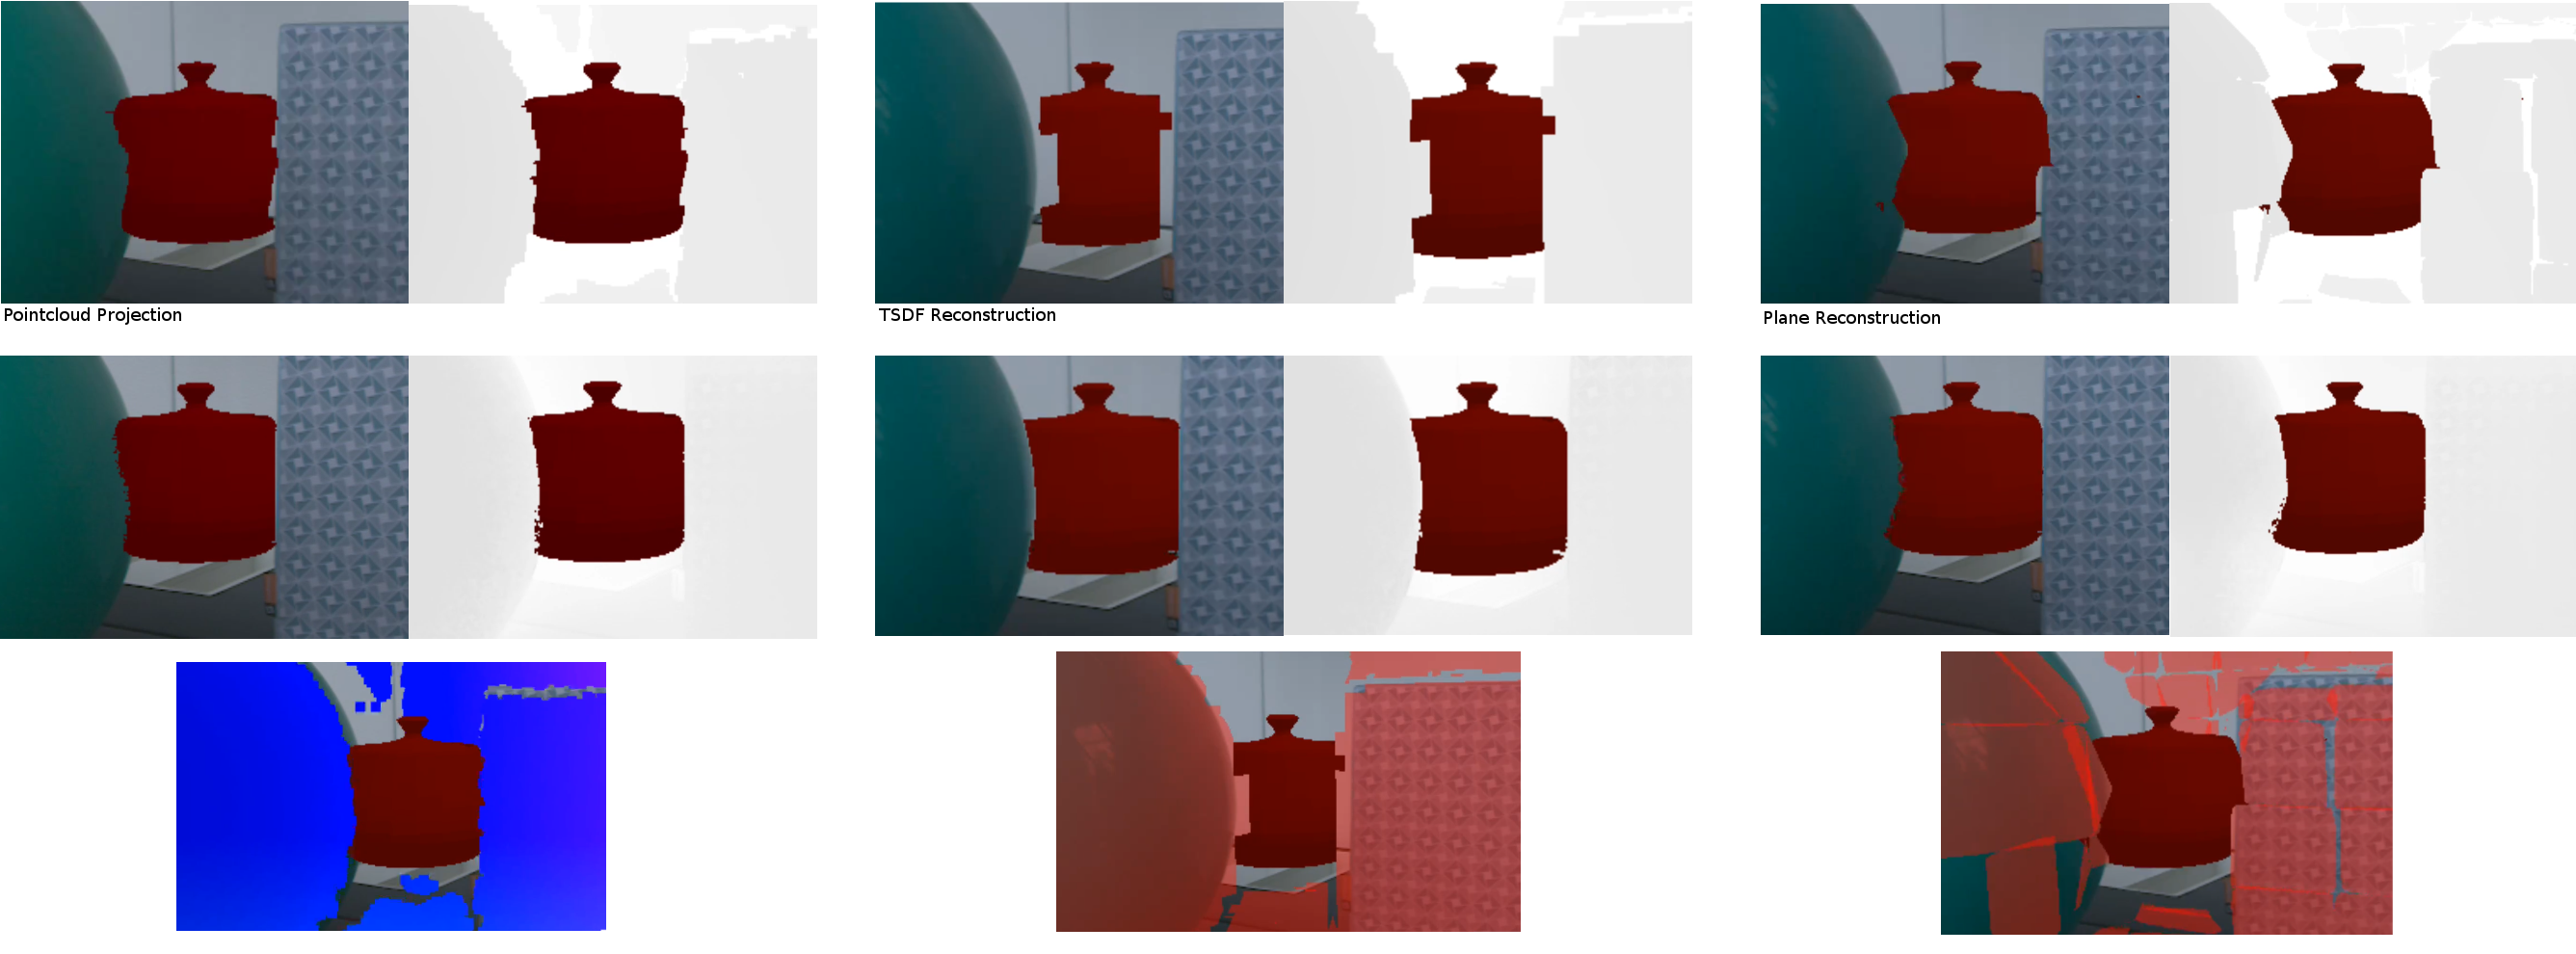
\includegraphics[width=1.0\textwidth]{content/images/evaluation/static_occlusion.png} 
  \caption{Ergebnisaufnahmen aus der ersten statischen Szene}
  \label{fig:static_occlusion}
\end{sidewaysfigure}

\begin{sidewaysfigure}[h]
  \centering
	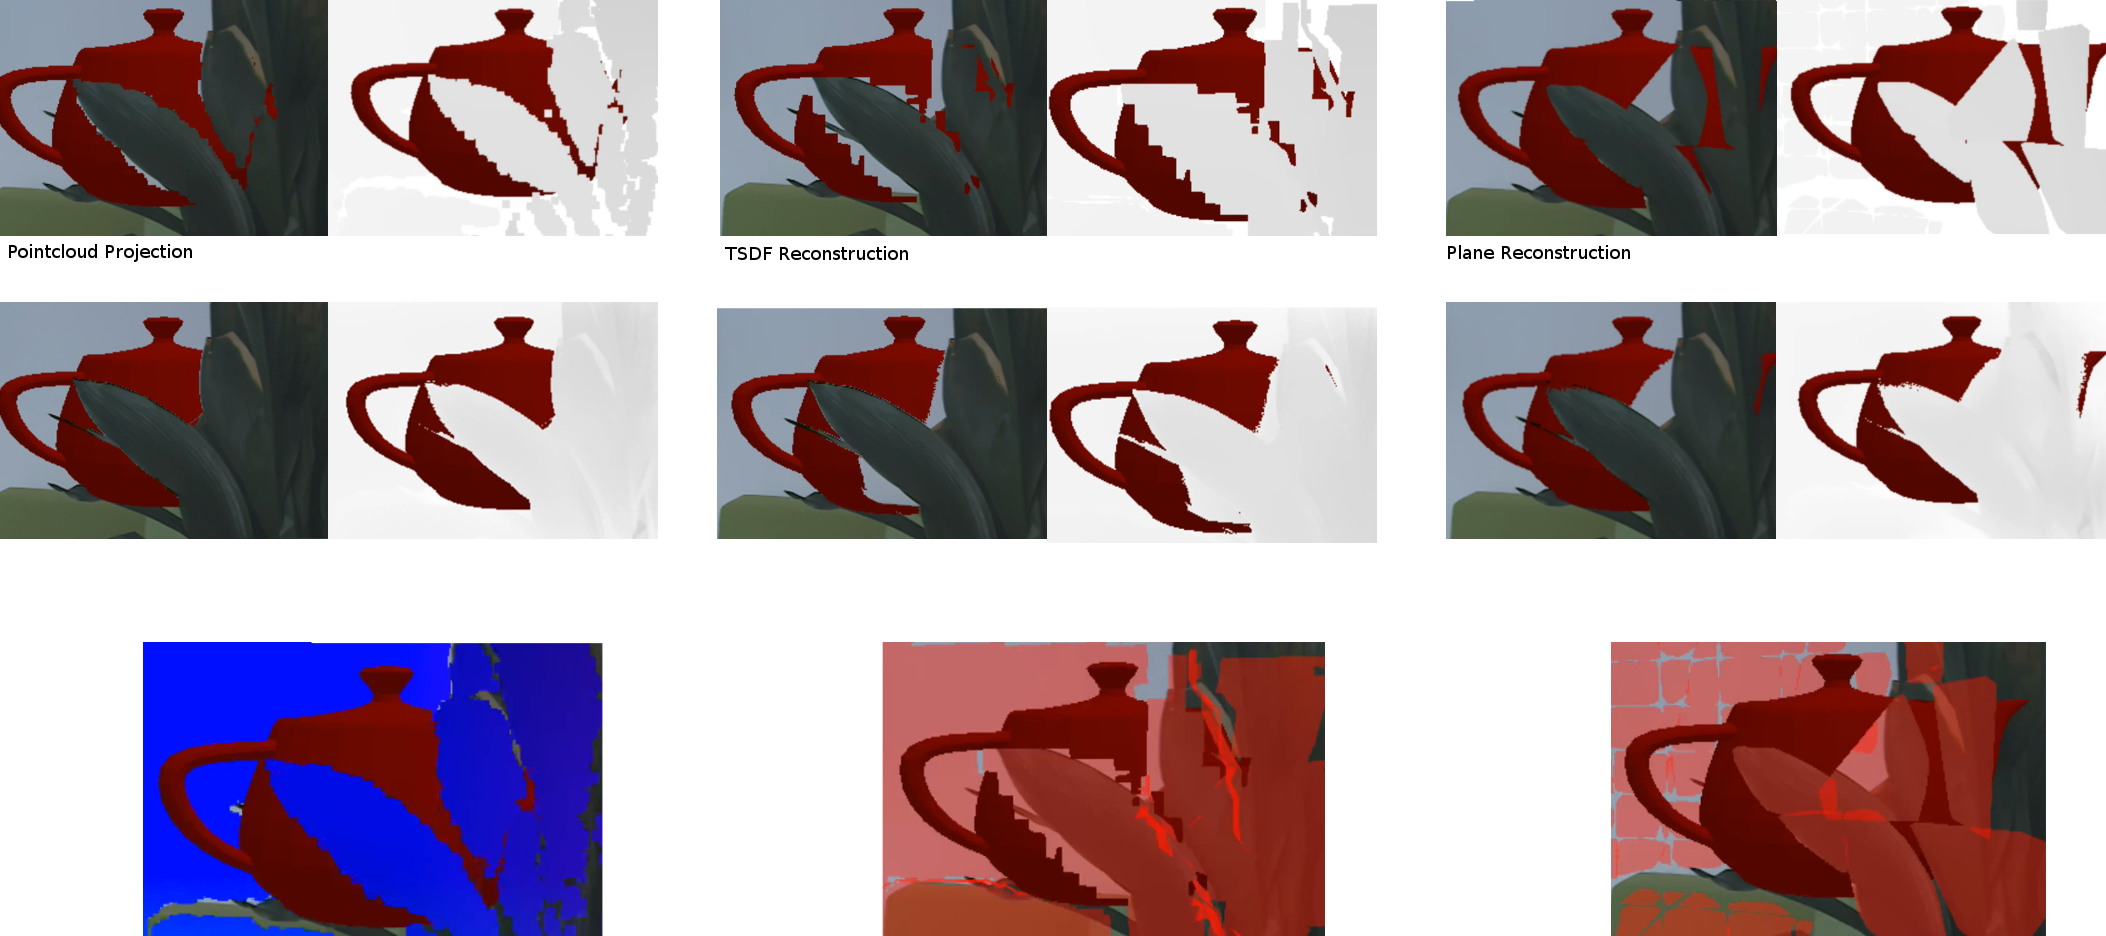
\includegraphics[width=1.0\textwidth]{content/images/evaluation/plant_occlusion.png} 
  \caption{Ergebnisaufnahmen aus der zweiten statischen Szene}
  \label{fig:plant_occlusion}
\end{sidewaysfigure}

\begin{sidewaysfigure}[h]
  \centering
	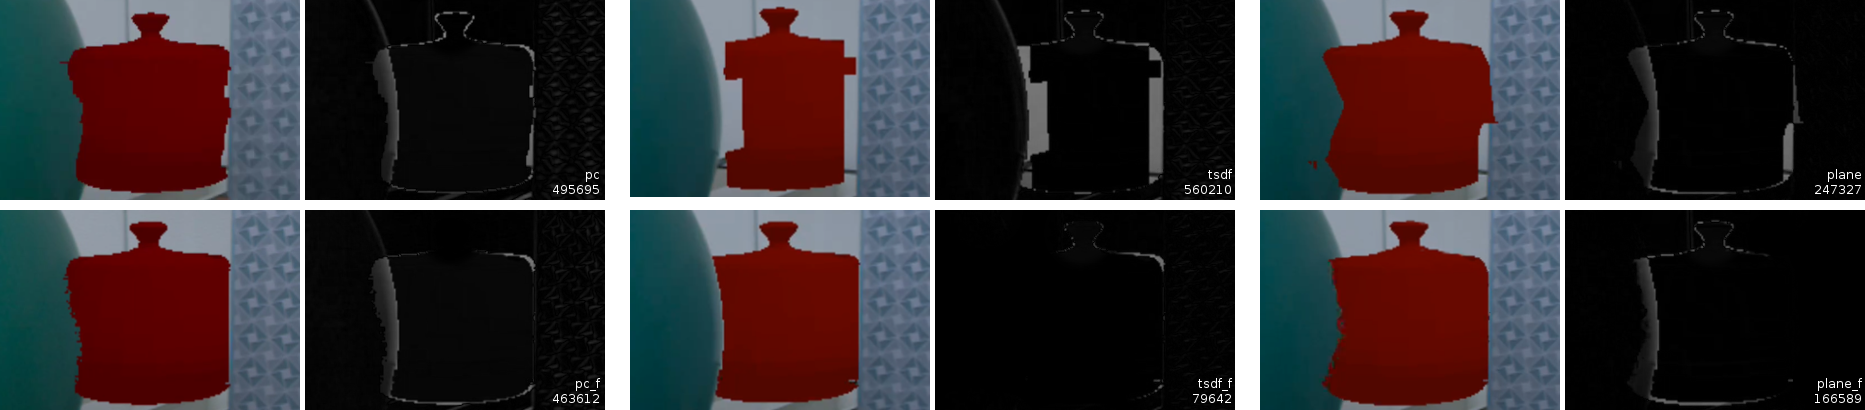
\includegraphics[width=1.0\textwidth]{content/images/evaluation/static_occlusion_results.png} 
	
\includegraphics[width=1.0\textwidth]{content/images/evaluation/spacer.png} 
	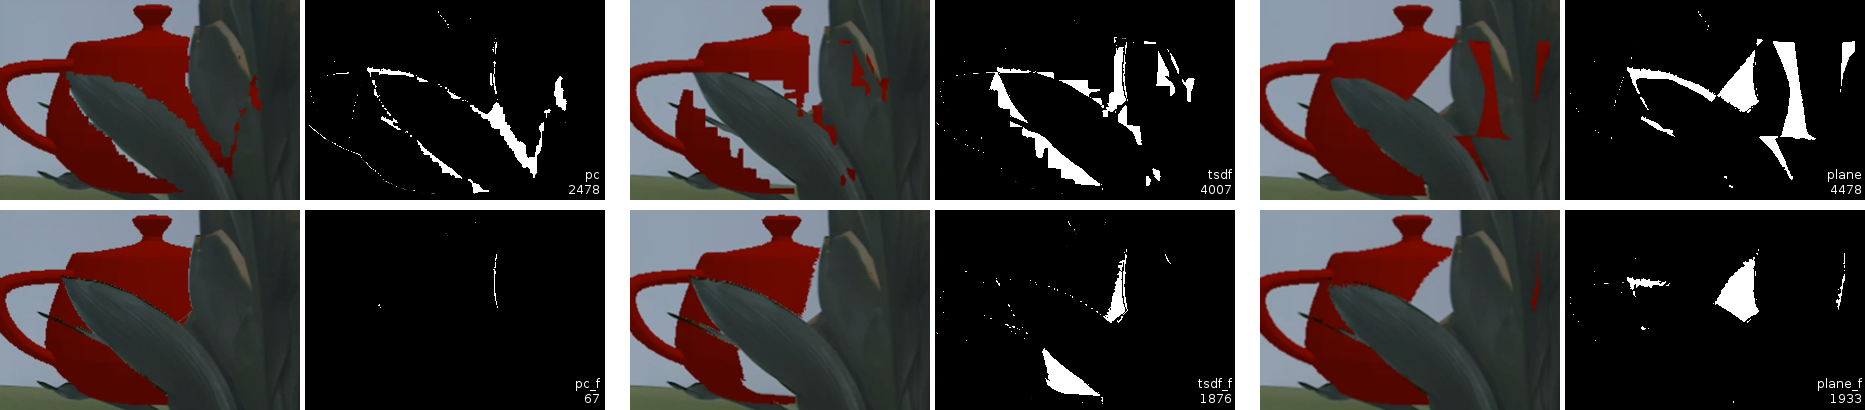
\includegraphics[width=1.0\textwidth]{content/images/evaluation/plant_occlusion_results.png} 
  \caption{Differenzbilder der Verfahren in ersten (oben) und zweiten Szene (unten)}
  \label{fig:static_occlusion_results}
\end{sidewaysfigure}
